% !TeX spellcheck = en_US
% !TeX encoding = UTF-8

\documentclass[aps, 10pt, a4paper]{article}
\usepackage{graphics, graphicx}
\usepackage{fancyvrb, enumerate}
\usepackage{amsmath, amssymb, amscd, amsfonts}
\usepackage{geometry}
\usepackage{multirow}
\usepackage{url}
\usepackage{tikz}
\usepackage{listings, listing}
\usepackage{color}
\usepackage{apacite}

\usetikzlibrary{shapes, arrows, calc, positioning}
\definecolor{codegreen}{rgb}{0, 0.6, 0}
\definecolor{codegray}{rgb}{0.5, 0.5, 0.5}
\definecolor{codepurple}{rgb}{0.58, 0, 0.82}
\definecolor{backcolour}{rgb}{0.95, 0.95, 0.92}
\lstdefinestyle{mystyle}
{
    backgroundcolor=\color{backcolour},   
    commentstyle=\color{codegreen},
    keywordstyle=\color{magenta},
    numberstyle=\tiny\color{codegray},
    stringstyle=\color{codepurple},
    basicstyle=\footnotesize,
    breakatwhitespace=false,         
    breaklines=true,                 
    captionpos=b,                    
    keepspaces=true,                 
    numbers=left,                    
    numbersep=5pt,                  
    showspaces=false,                
    showstringspaces=false,
    showtabs=false,                  
    tabsize=2,
    frame=single
}
\lstset{style=mystyle}
\tikzstyle{decision} = [diamond, draw, fill=blue!20, text width=4.5em, text badly centered, node distance=3cm, inner sep=0pt]
\tikzstyle{block} = [rectangle, draw, fill=blue!20, text width=5em, text centered, rounded corners, minimum height=2em]
\tikzstyle{line} = [draw, -latex']
\tikzstyle{cloud} = [draw, ellipse, fill=red!20, node distance=5em, minimum height=2em]
\tikzset
{
    -|-/.style=
    {
        to path=
        {
            (\tikztostart) -| ($(\tikztostart)!#1!(\tikztotarget)$) |- (\tikztotarget)
            \tikztonodes
        }
    },
    -|-/.default=0.5,
    |-|/.style=
    {
        to path=
        {
            (\tikztostart) |- ($(\tikztostart)!#1!(\tikztotarget)$) -| (\tikztotarget)
            \tikztonodes
        }
    },
    |-|/.default=0.5,
}
\geometry
{
    top = 20mm,
    bottom = 20mm,
    left = 20mm,
    right = 20mm
}

\title{Visualization Term Project}
\author{20141087 Ryeongyun Kim \and 20161206 Jaewoong Lee}
\date{\today}

\begin{document}
    \maketitle
    \newpage
    
    \tableofcontents
    \listoftables
    \listoffigures
    \newpage
    
    \section{Introduction}
    
    \section{Materials}
        \subsection{Building Layout}
            \subsubsection{Basic}
                \begin{figure}[htbp]
                    \centering
                    $\begin{array}{ccc}
                        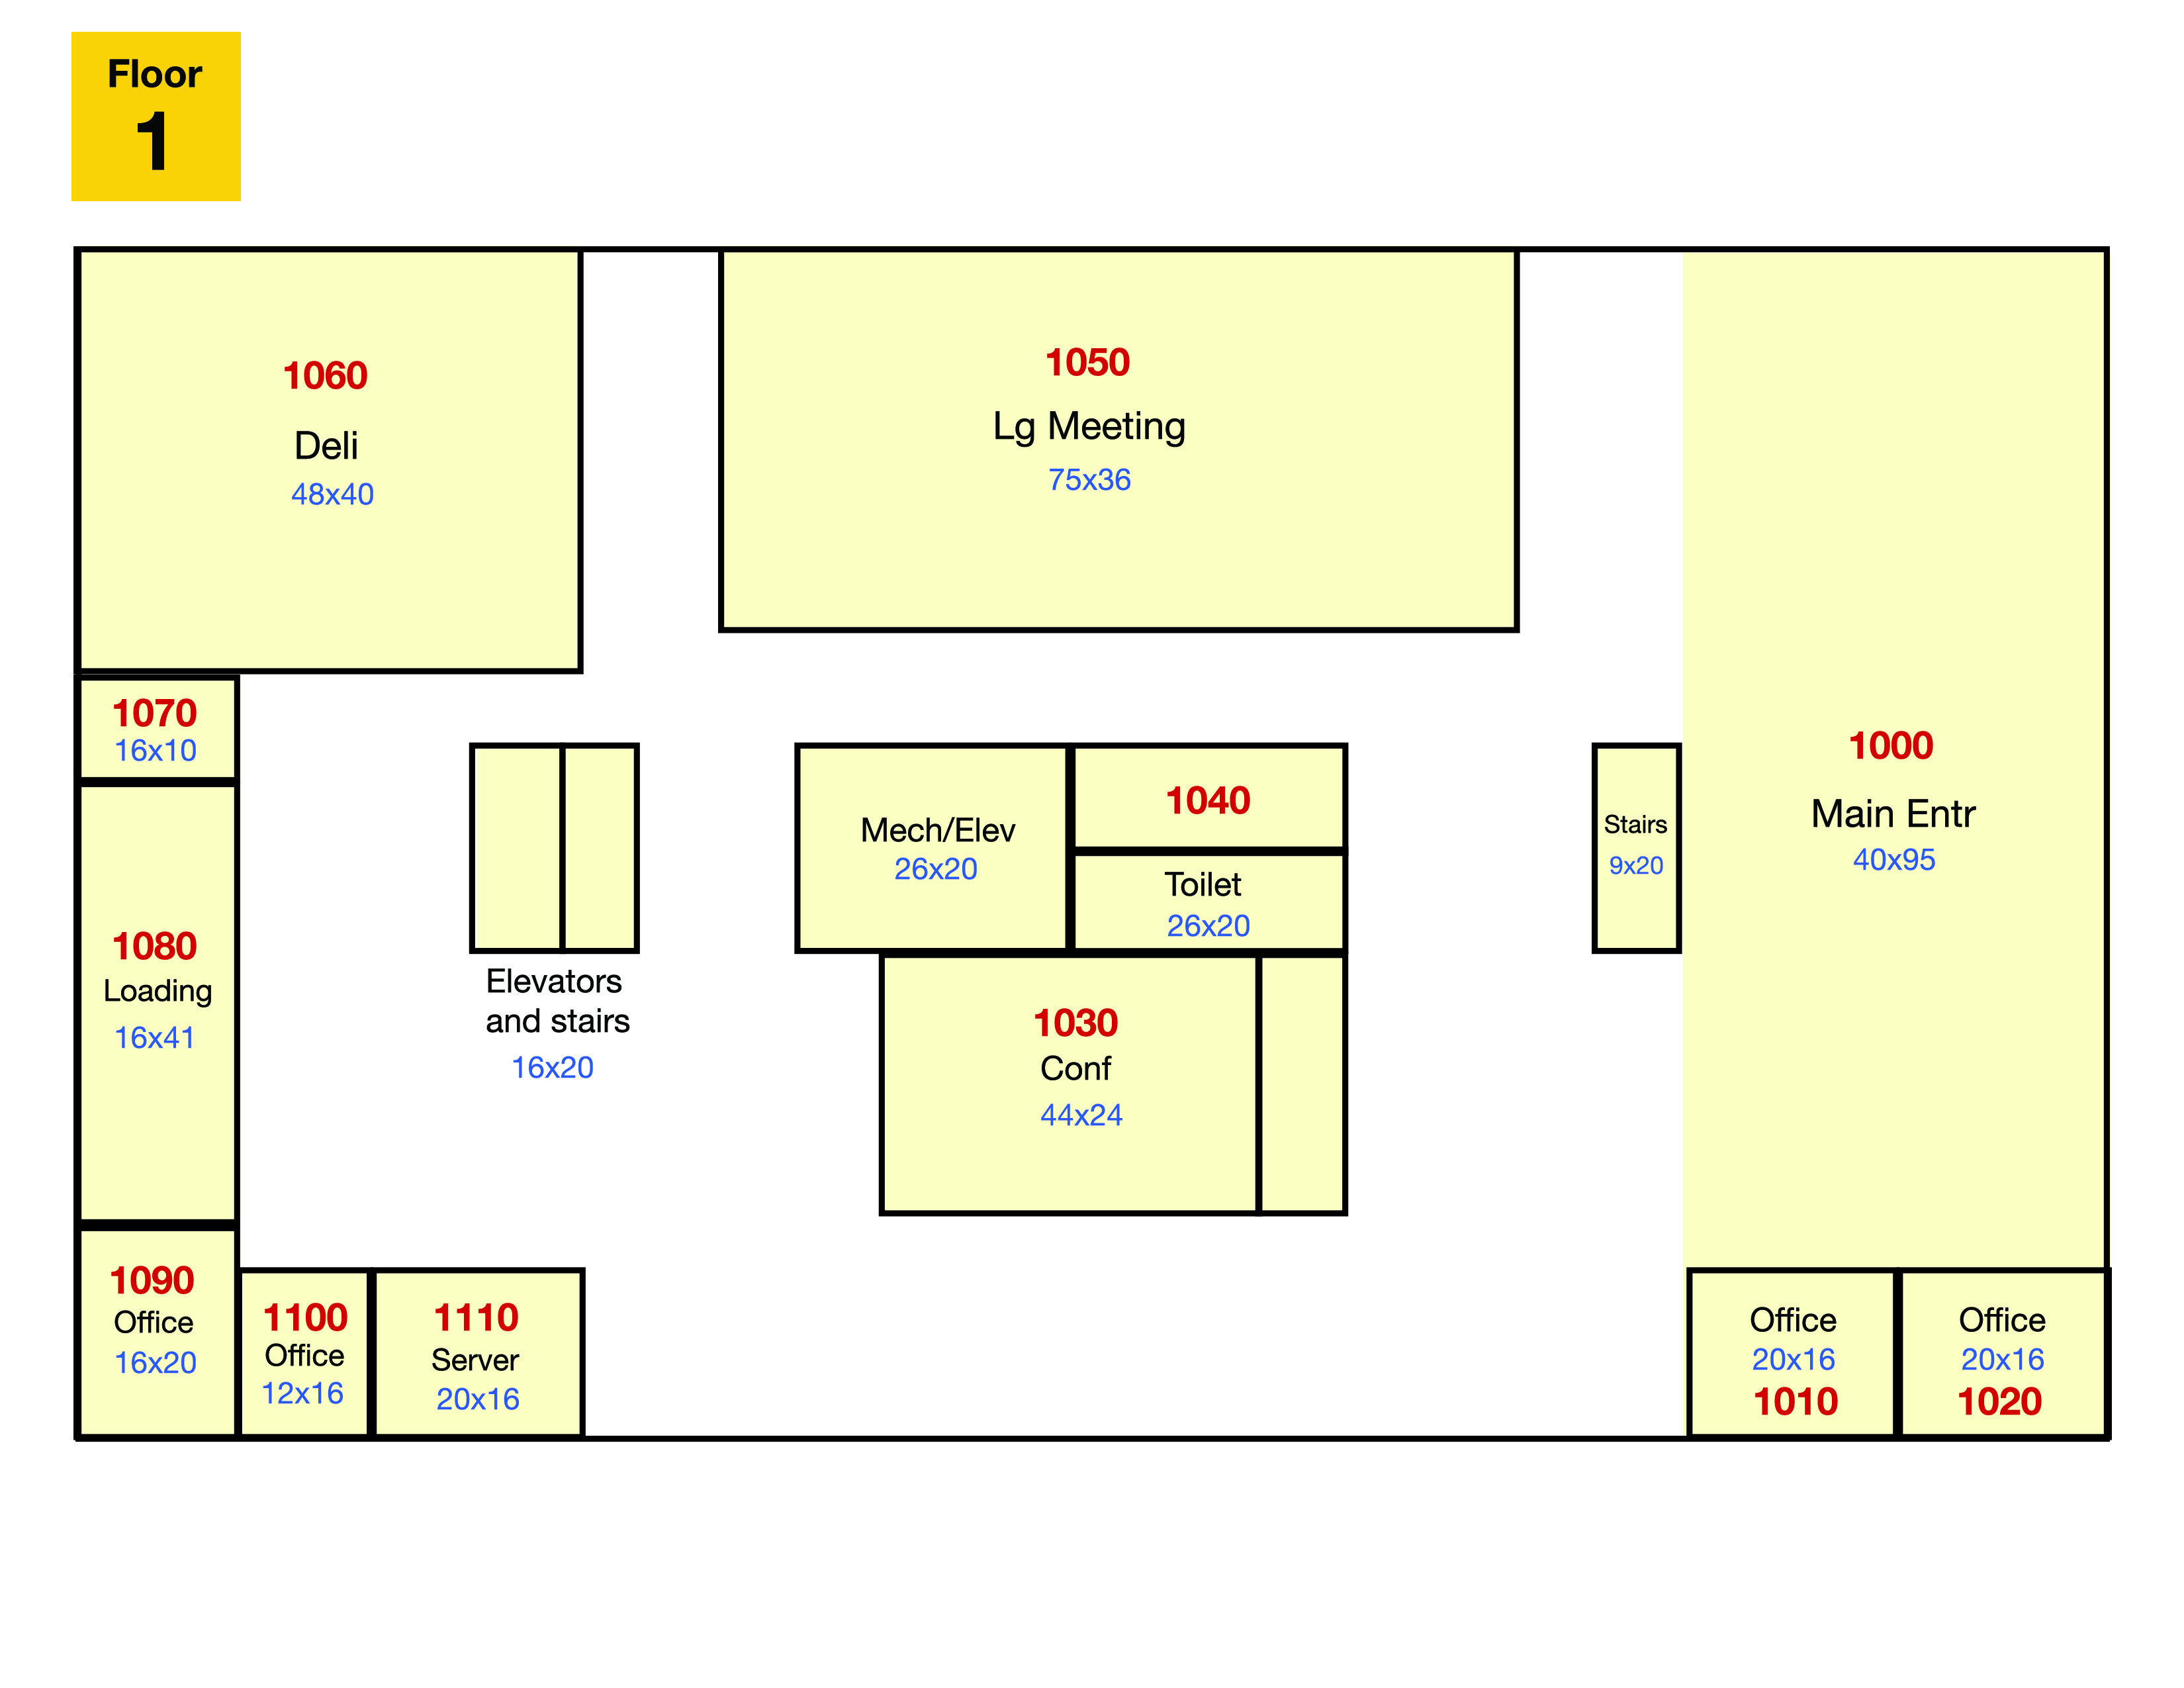
\includegraphics[width=0.3 \linewidth]{figures/basic1.jpg}
                        &
                        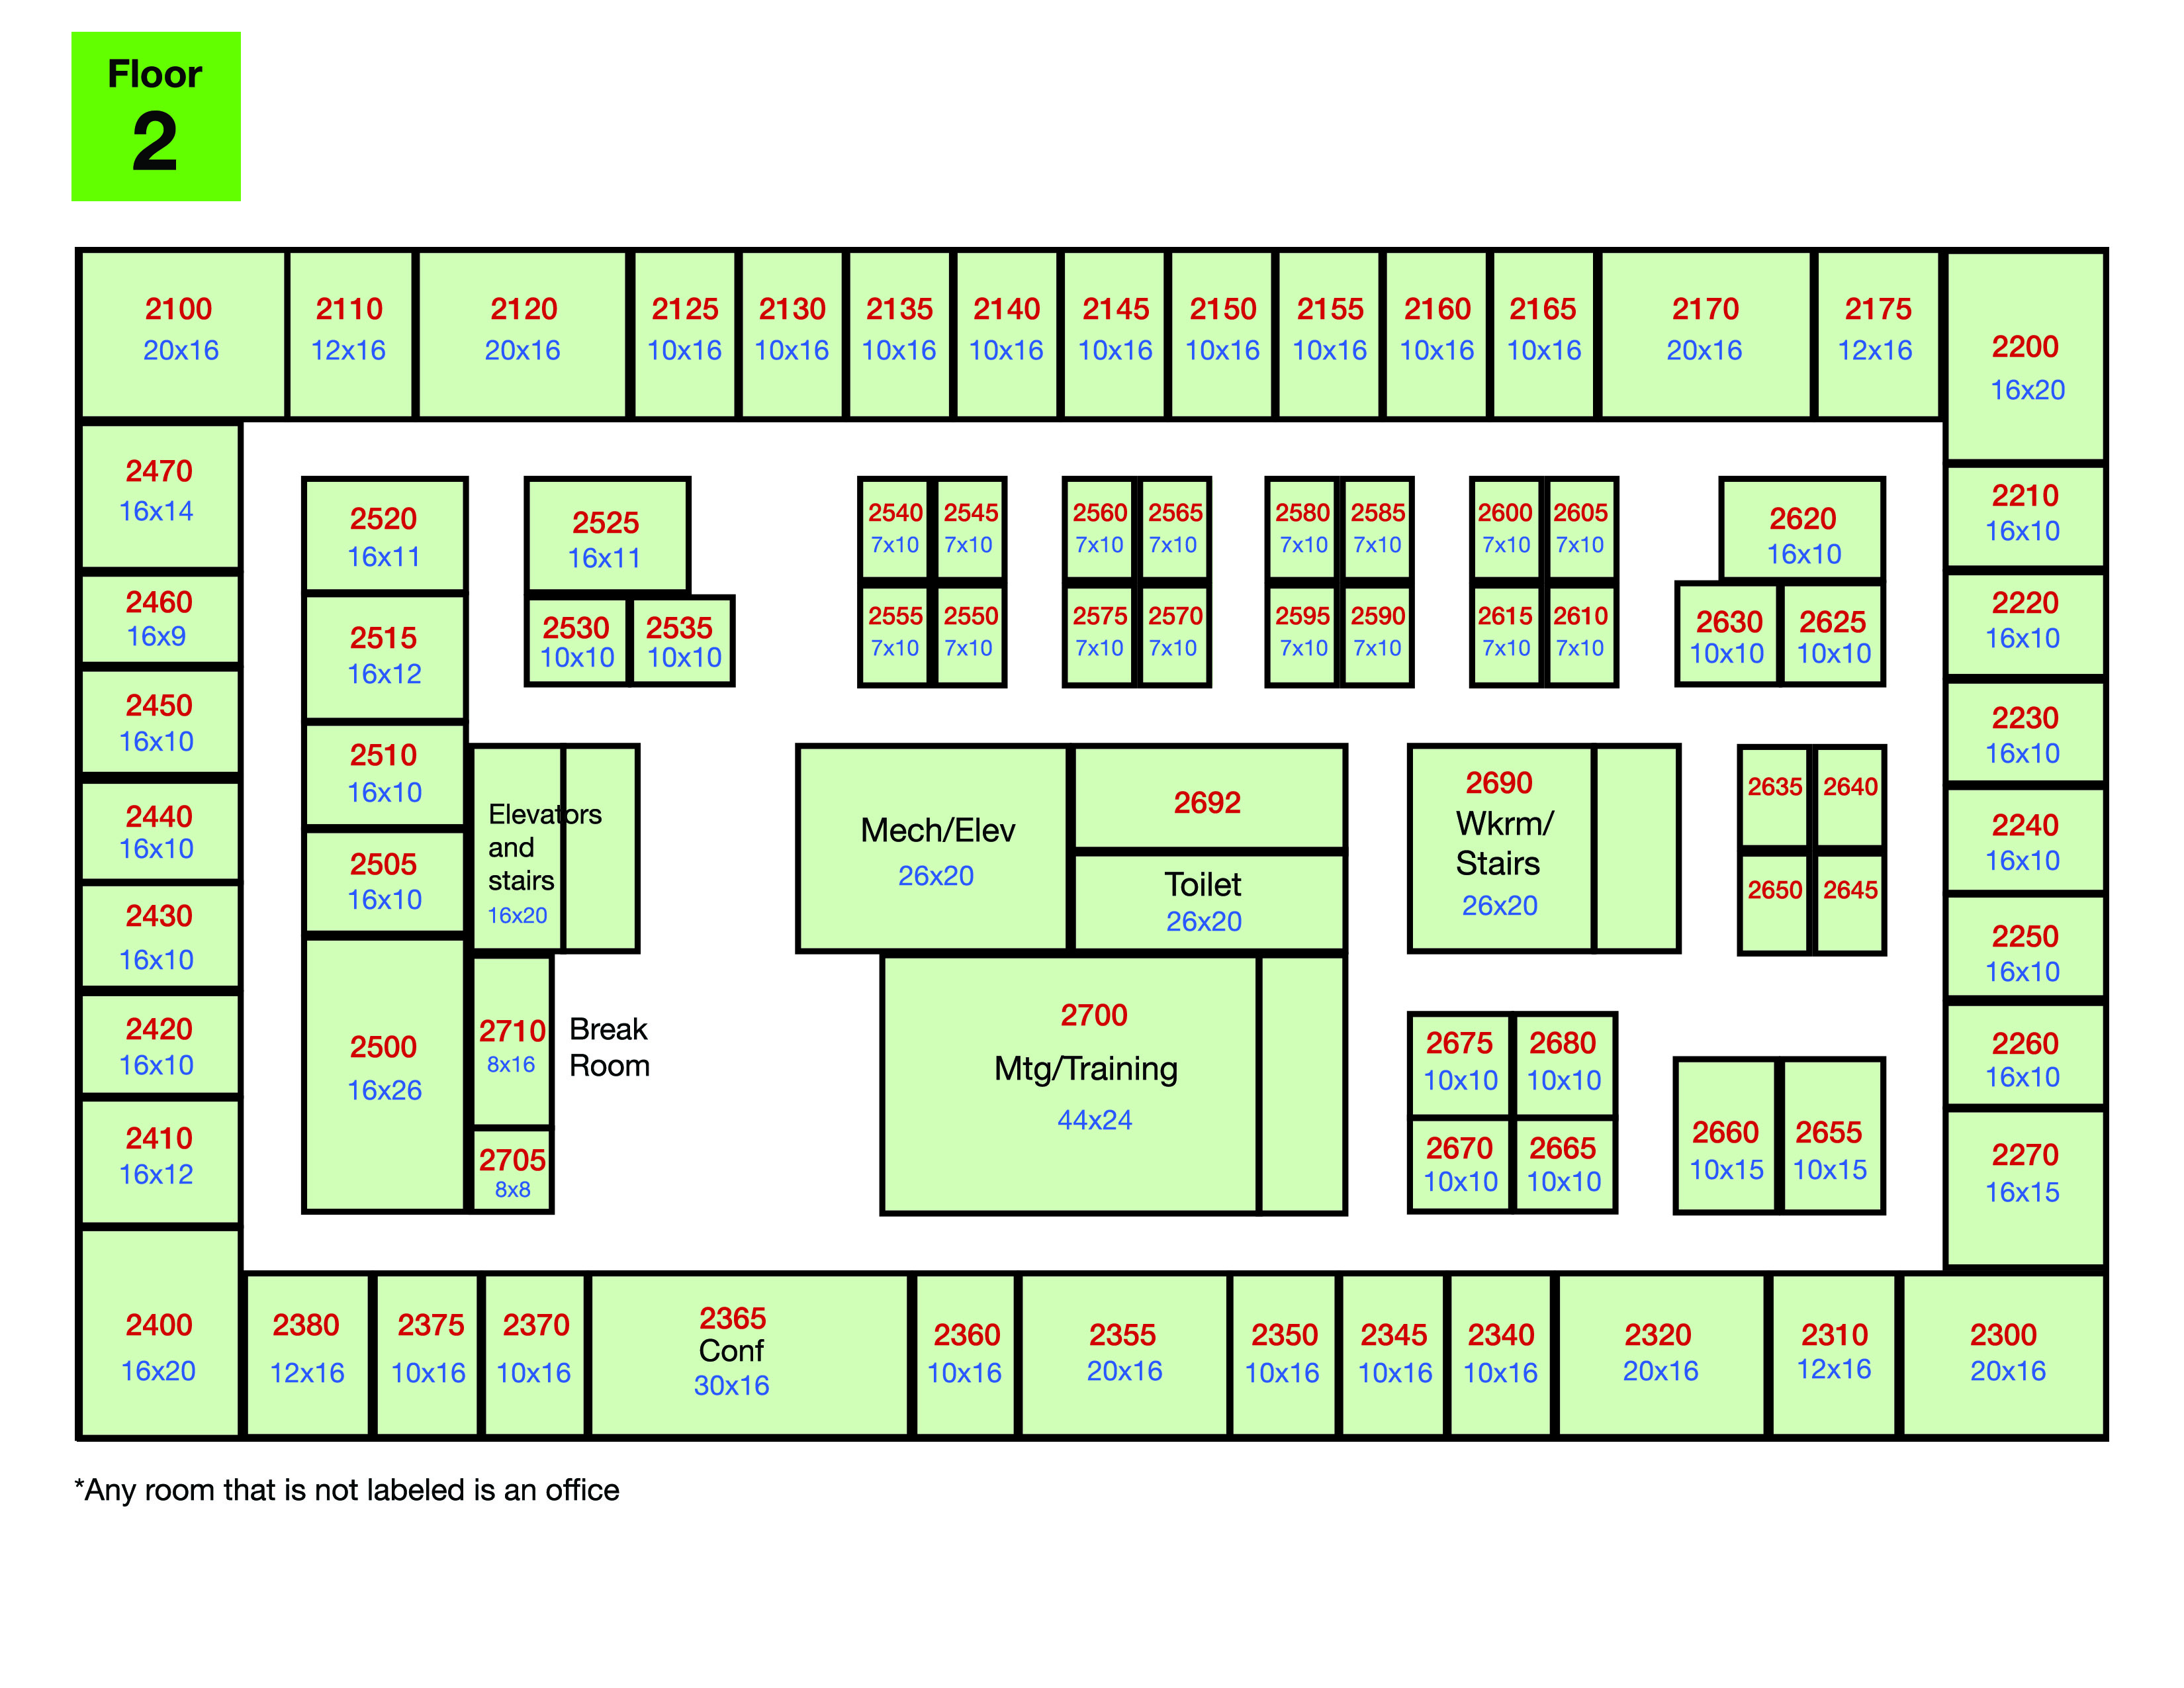
\includegraphics[width=0.3 \linewidth]{figures/basic2.jpg}
                        &
                        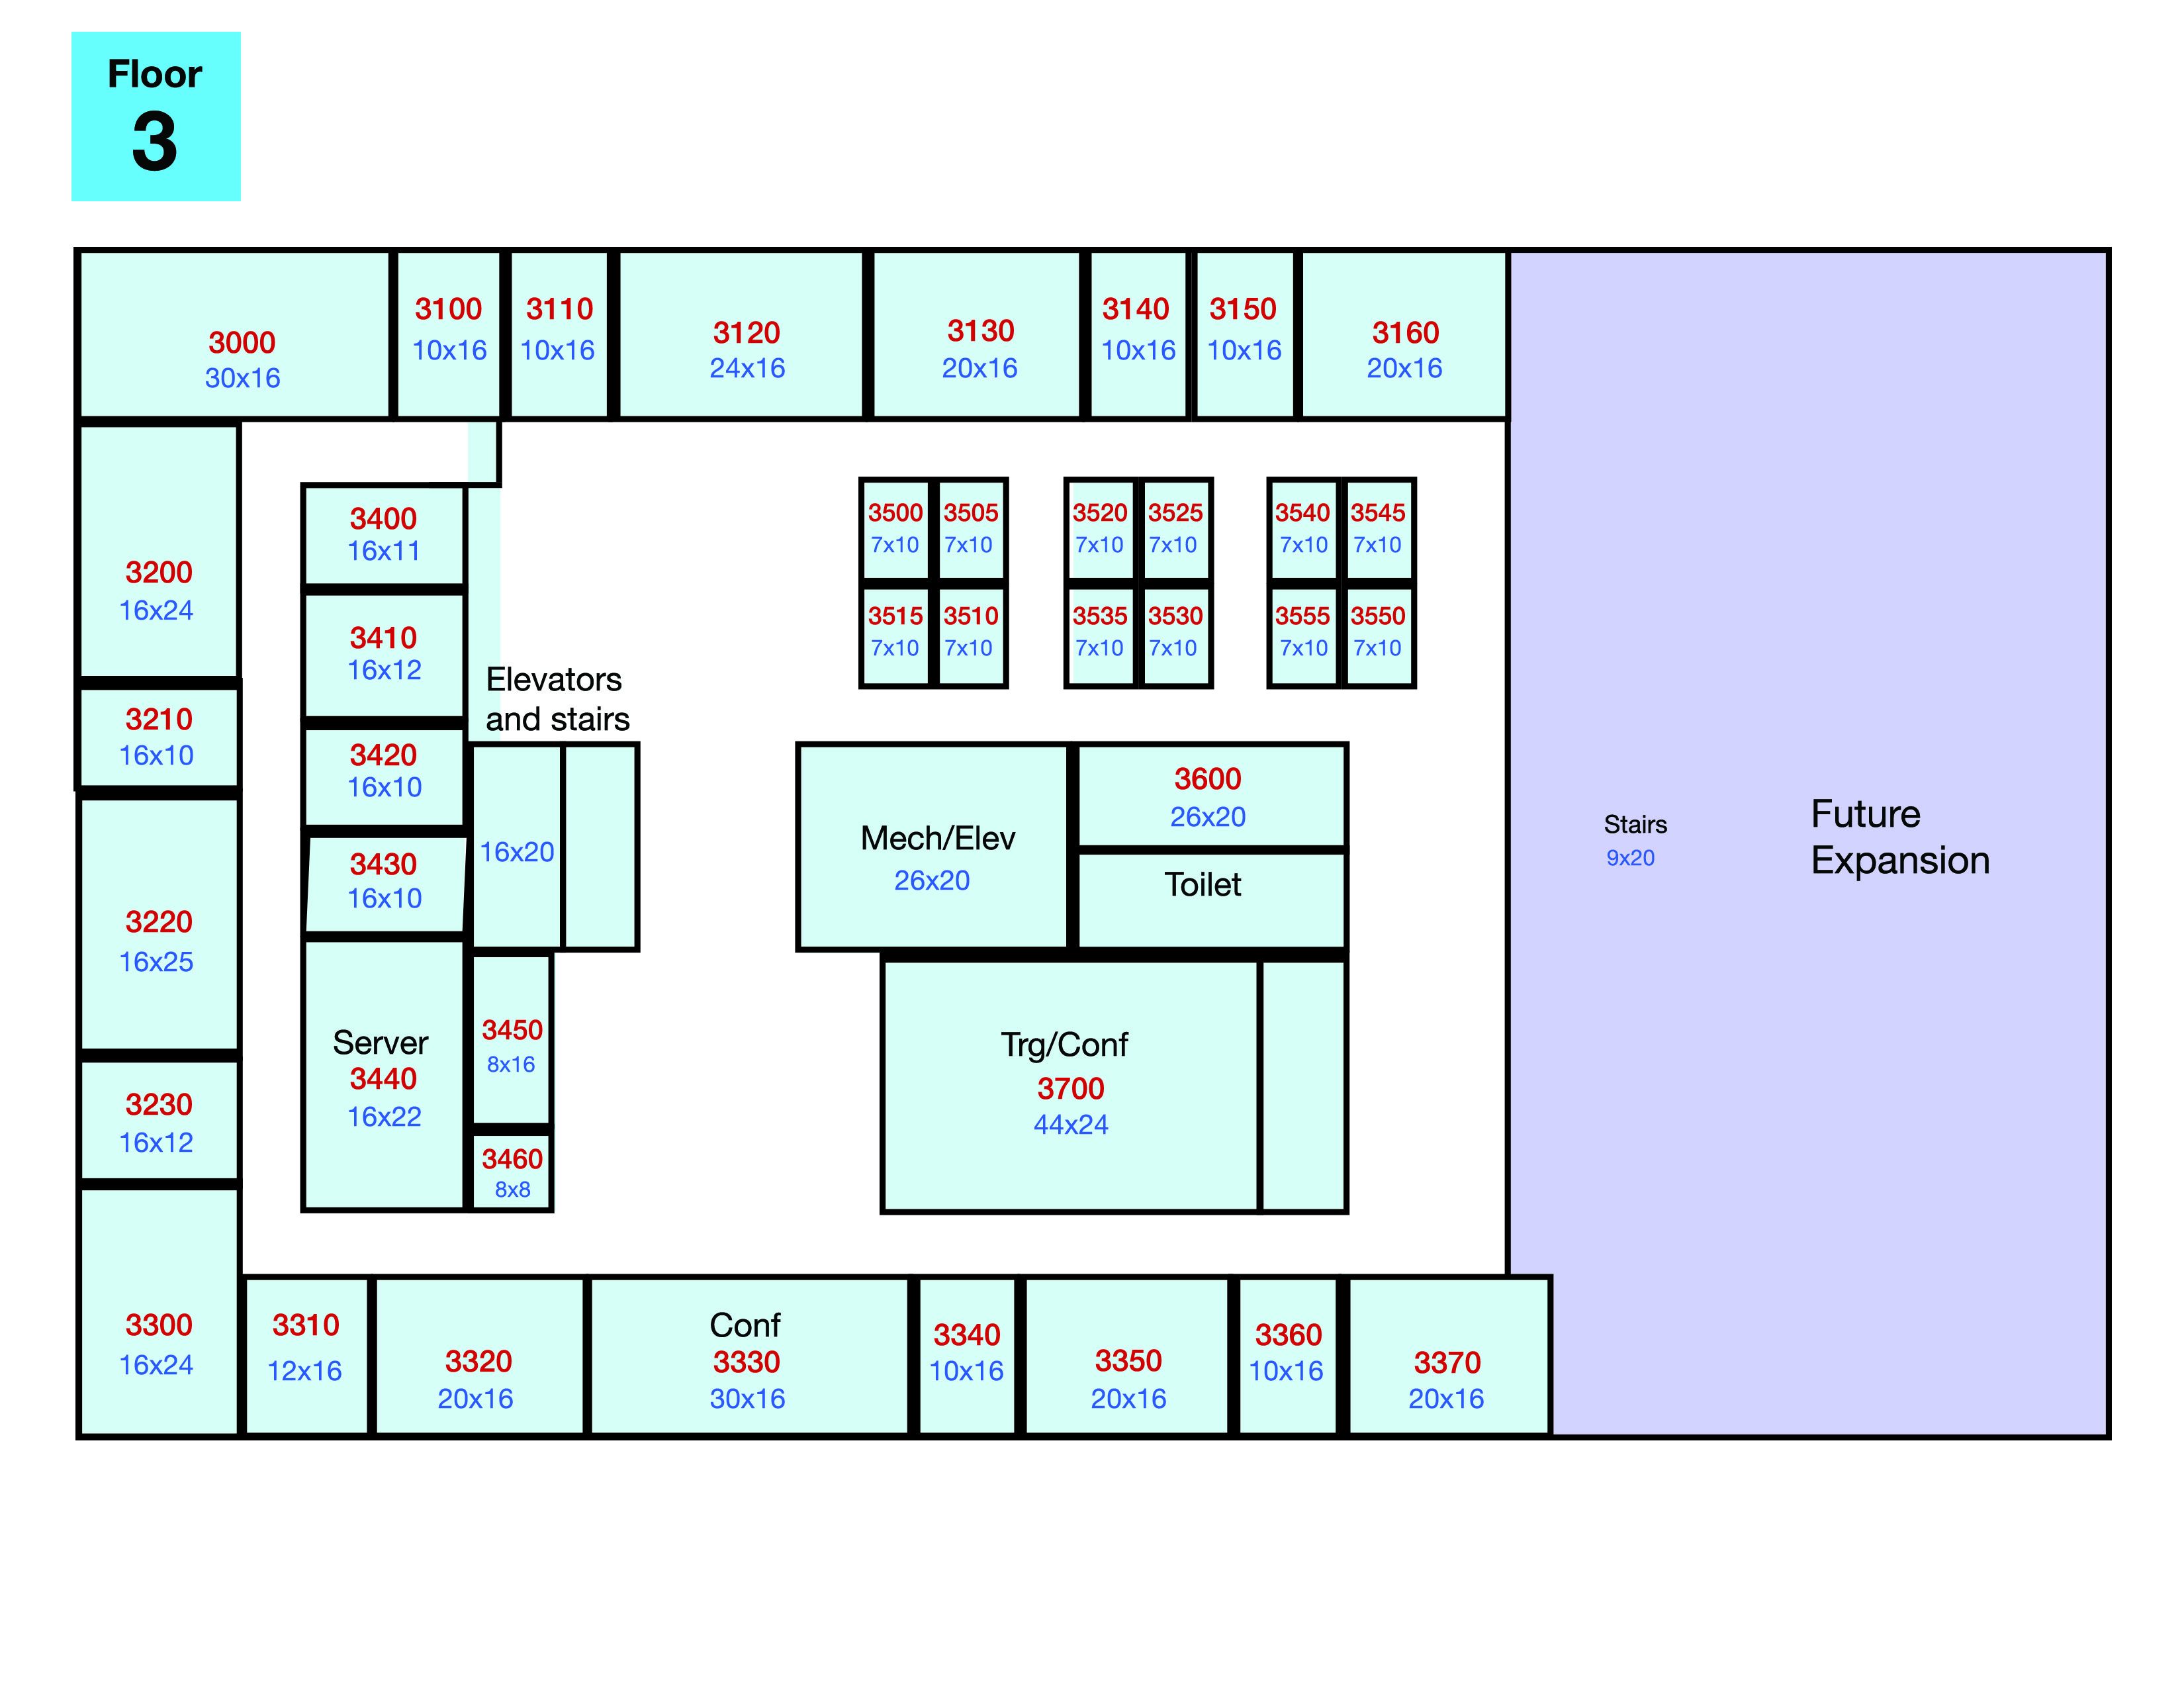
\includegraphics[width=0.3 \linewidth]{figures/basic3.jpg}
                        \\
                        
                        \mbox{(a) First Floor} & \mbox{(b) Second Floor} & \mbox{Third Floor} \\
                    \end{array}$
                    \caption{Main Layout of the building}
                    \label{fig:main}
                \end{figure}
            
                The main layout of this building is as figure \ref{fig:main}. 
                
                \begin{figure}[htbp]
                    \centering
                    $\begin{array}{ccc}
                        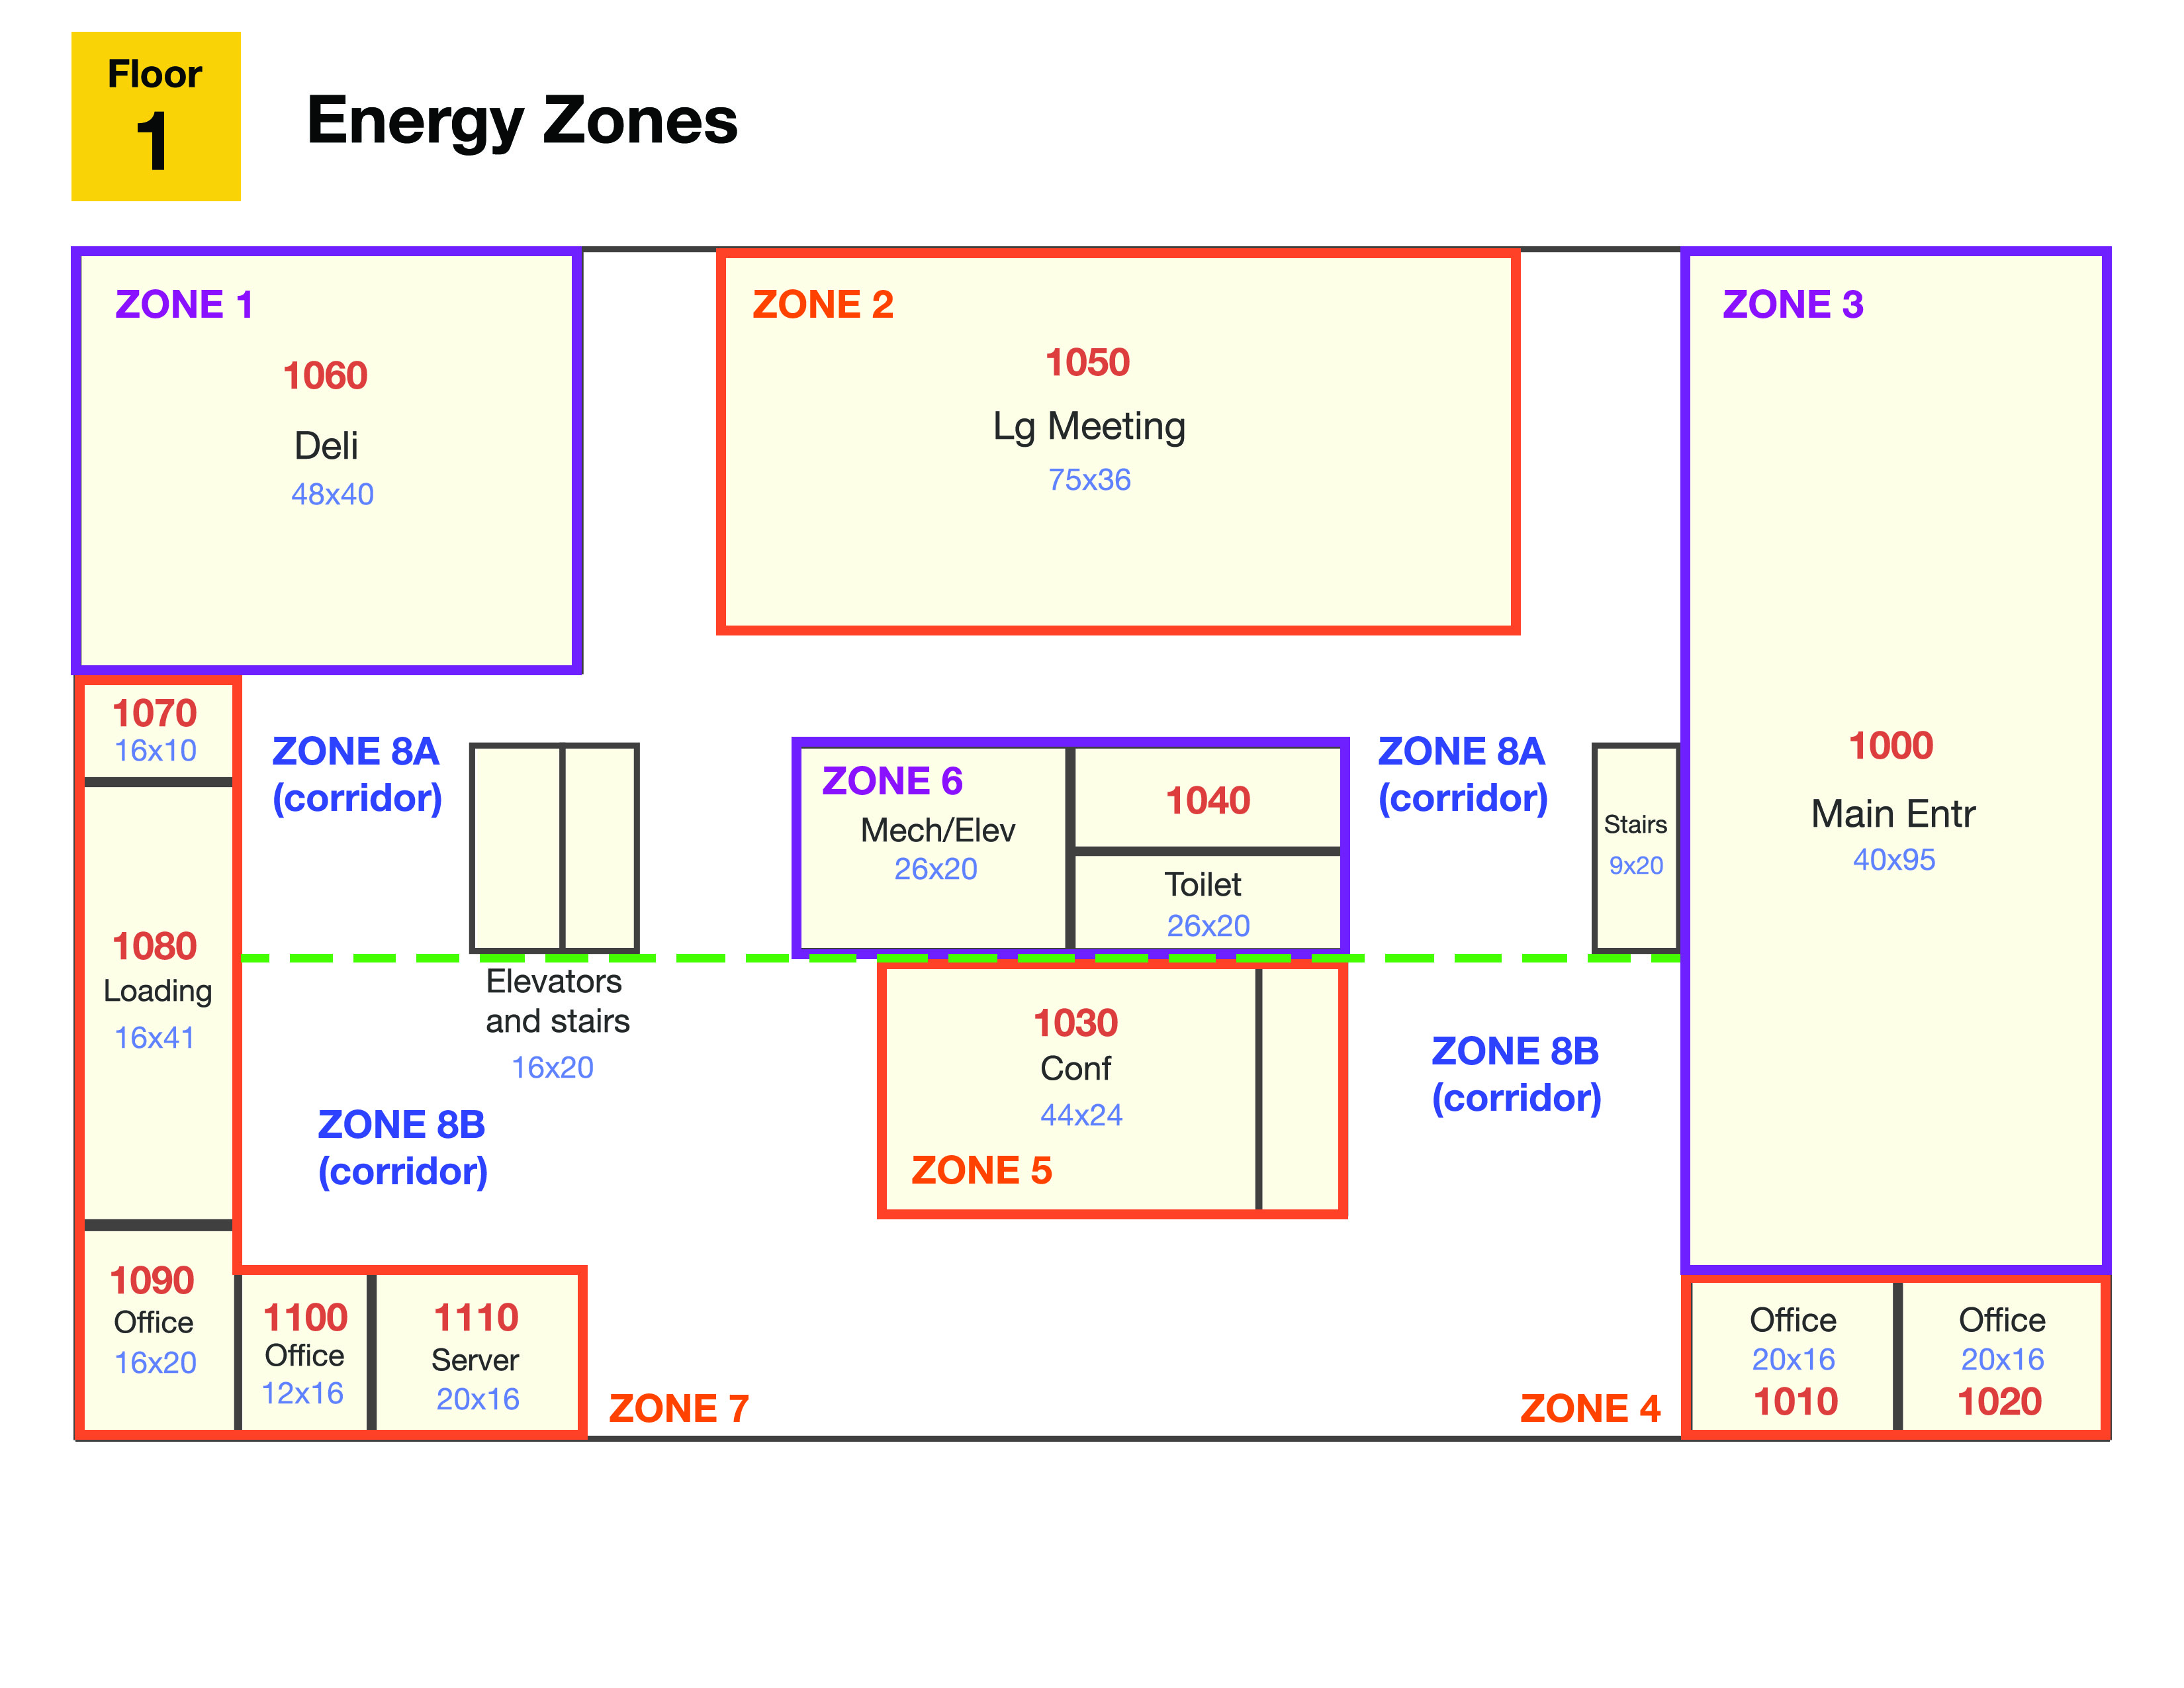
\includegraphics[width=0.3 \linewidth]{figures/energy1.jpg}
                        &
                        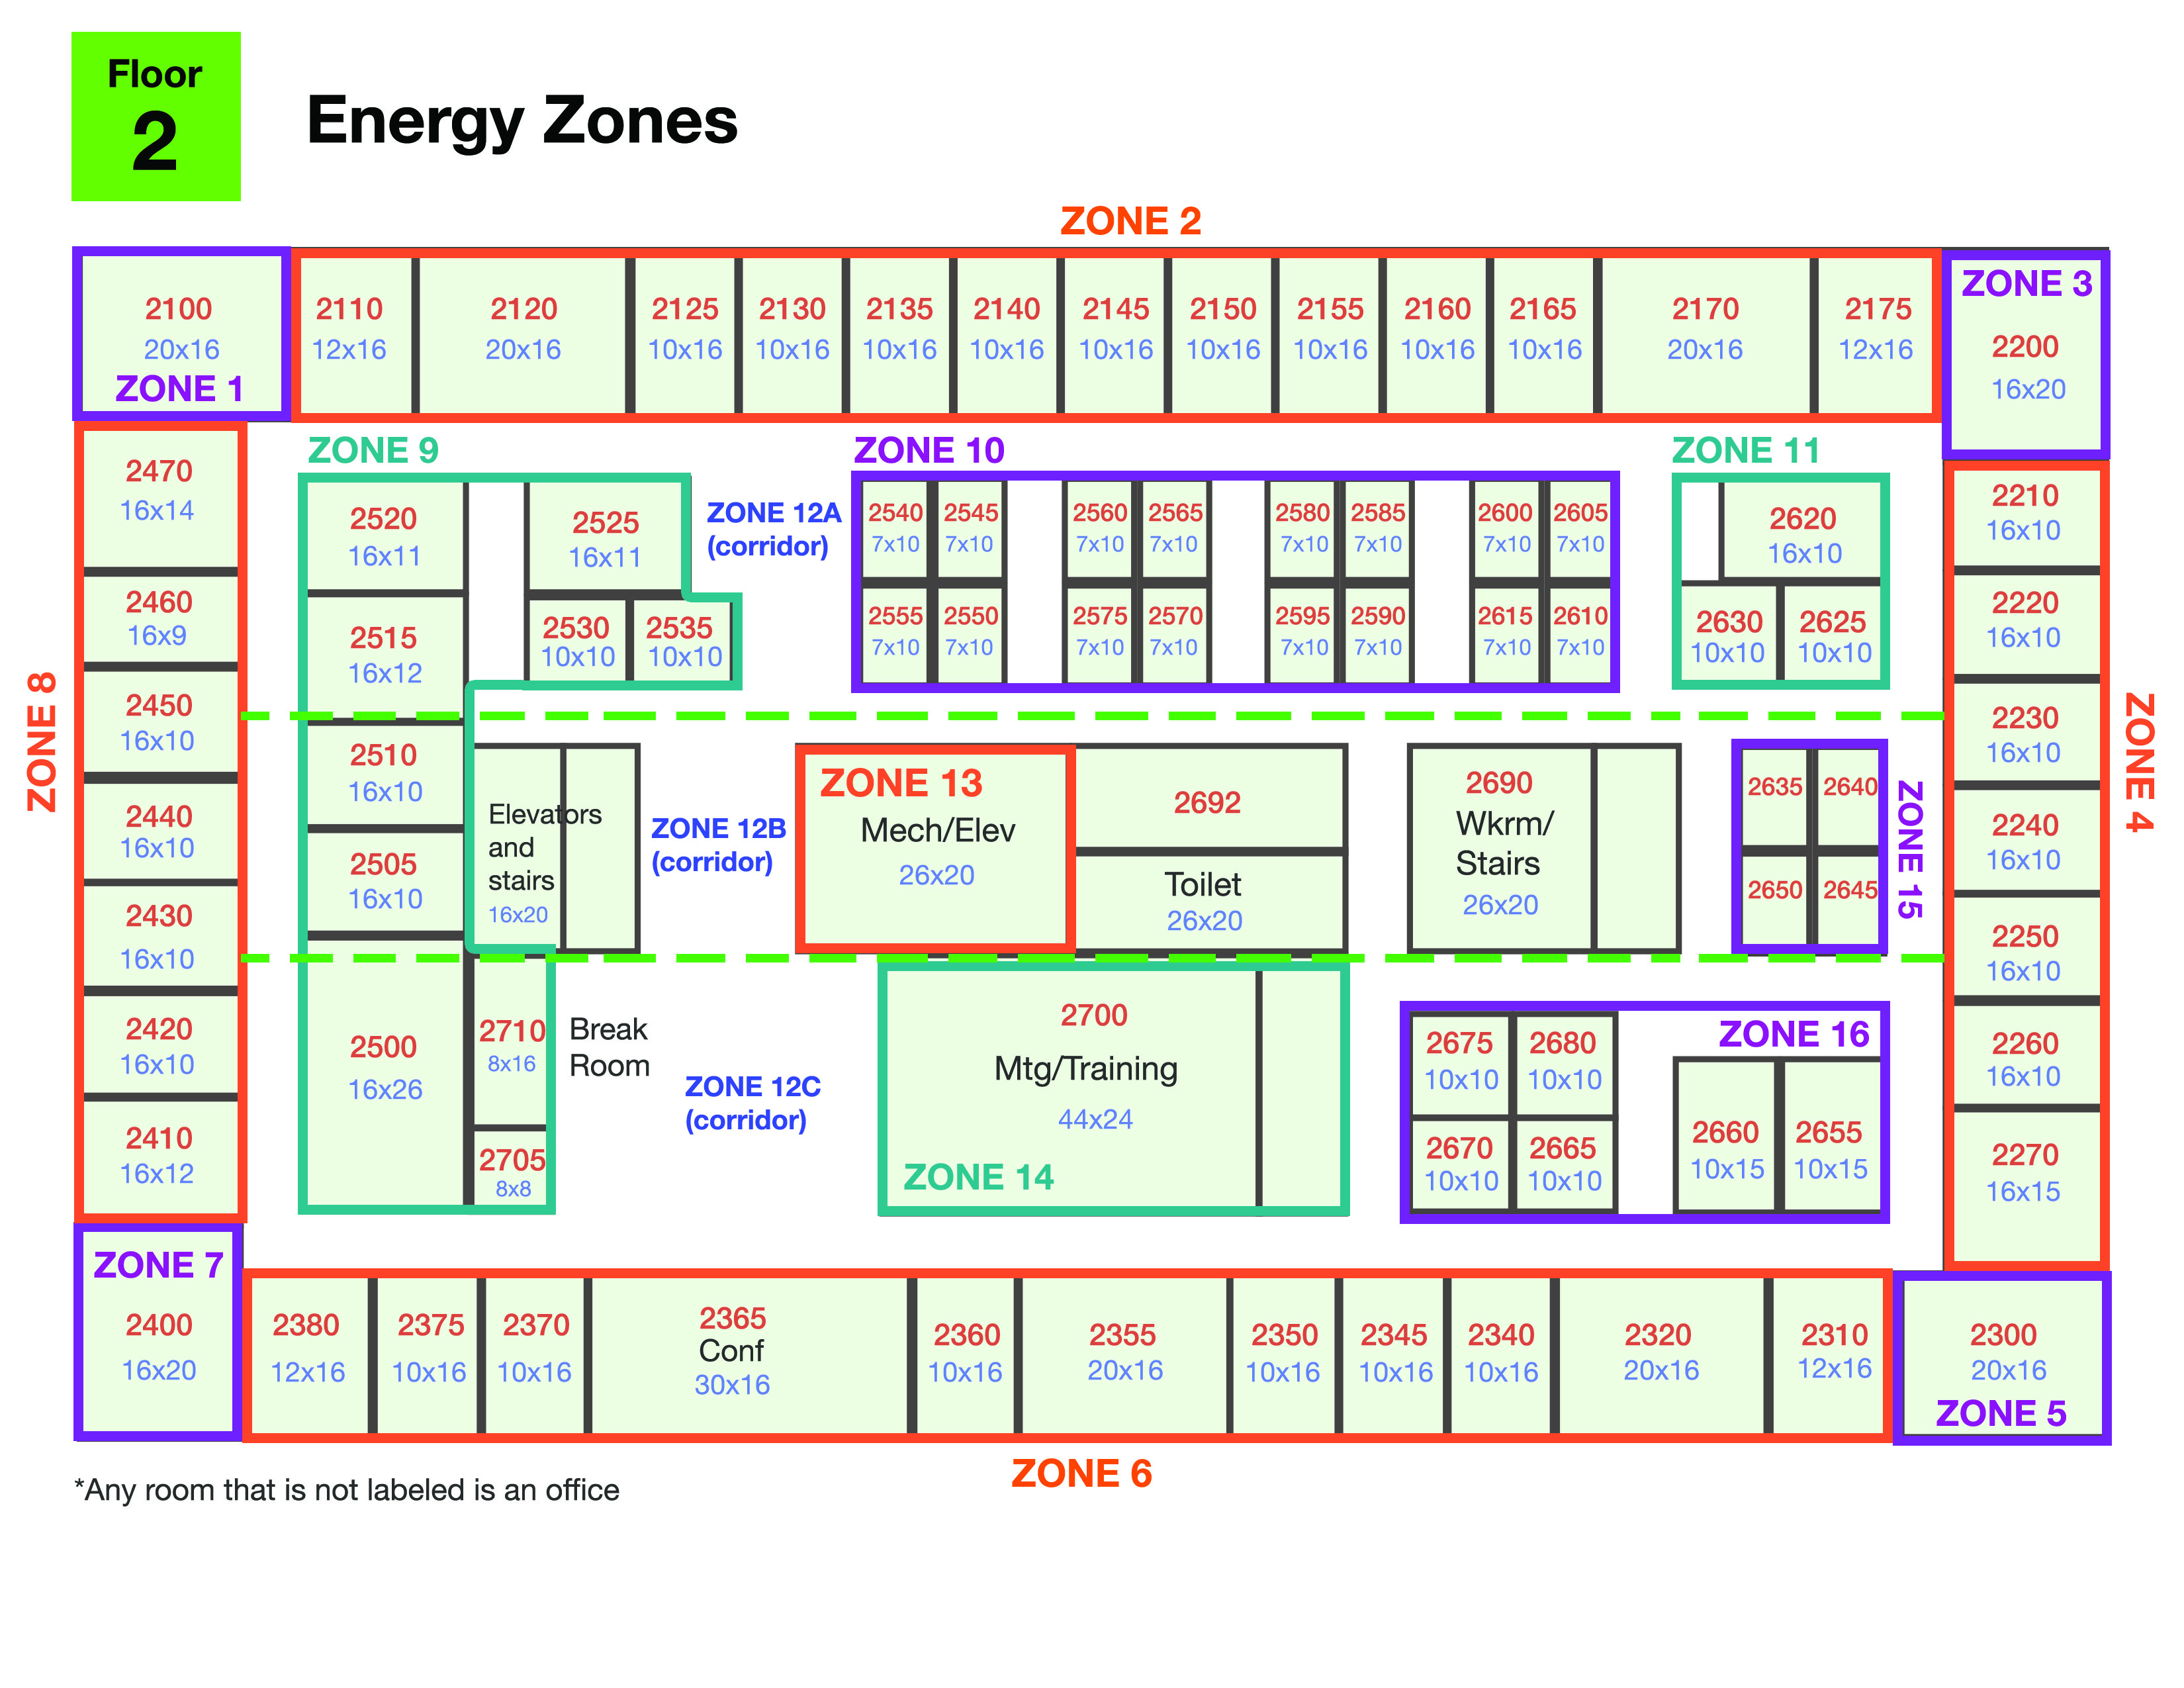
\includegraphics[width=0.3 \linewidth]{figures/energy2.jpg}
                        &
                        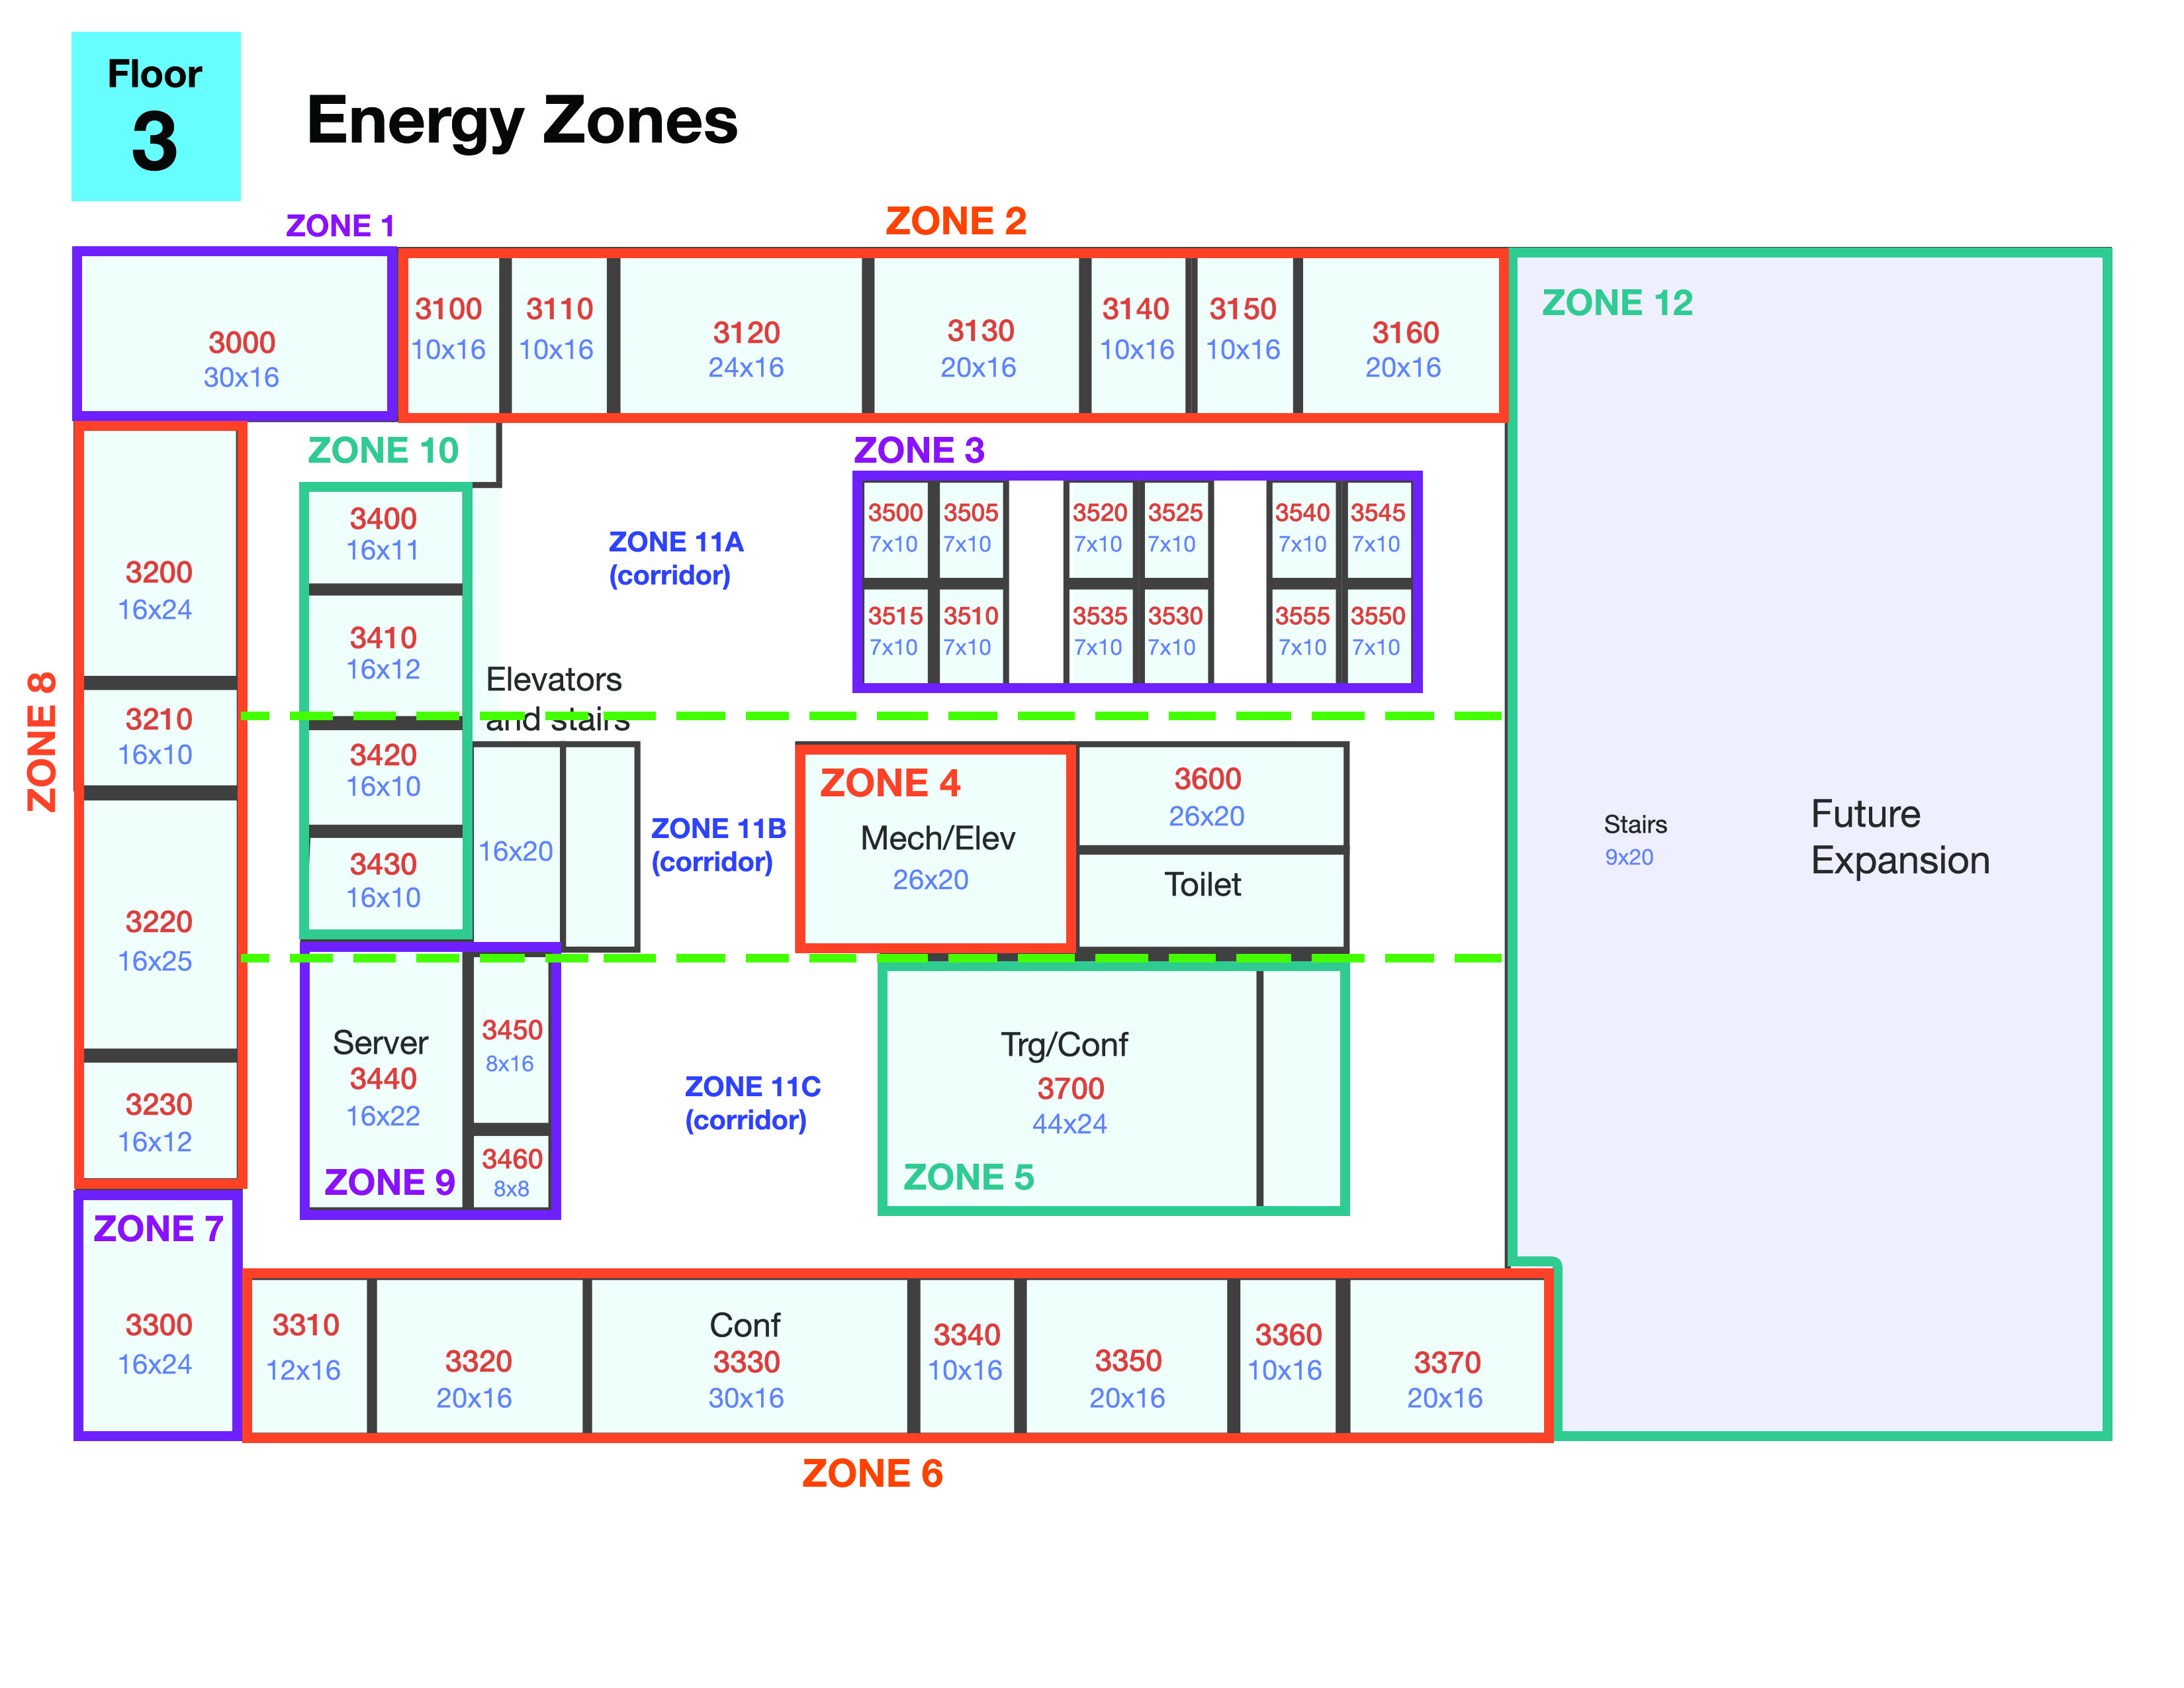
\includegraphics[width=0.3 \linewidth]{figures/energy3.jpg}
                        \\
                        
                        \mbox{(a) First Floor} & \mbox{(b) Second Floor} & \mbox{Third Floor} \\
                    \end{array}$
                    \caption{Energy Zone of the Building}
                    \label{fig:energy}
                \end{figure}
            
                The energy zone of this building is as figure \ref{fig:energy}. 
                
                \begin{figure}[htbp]
                    \centering
                    $\begin{array}{ccc}
                        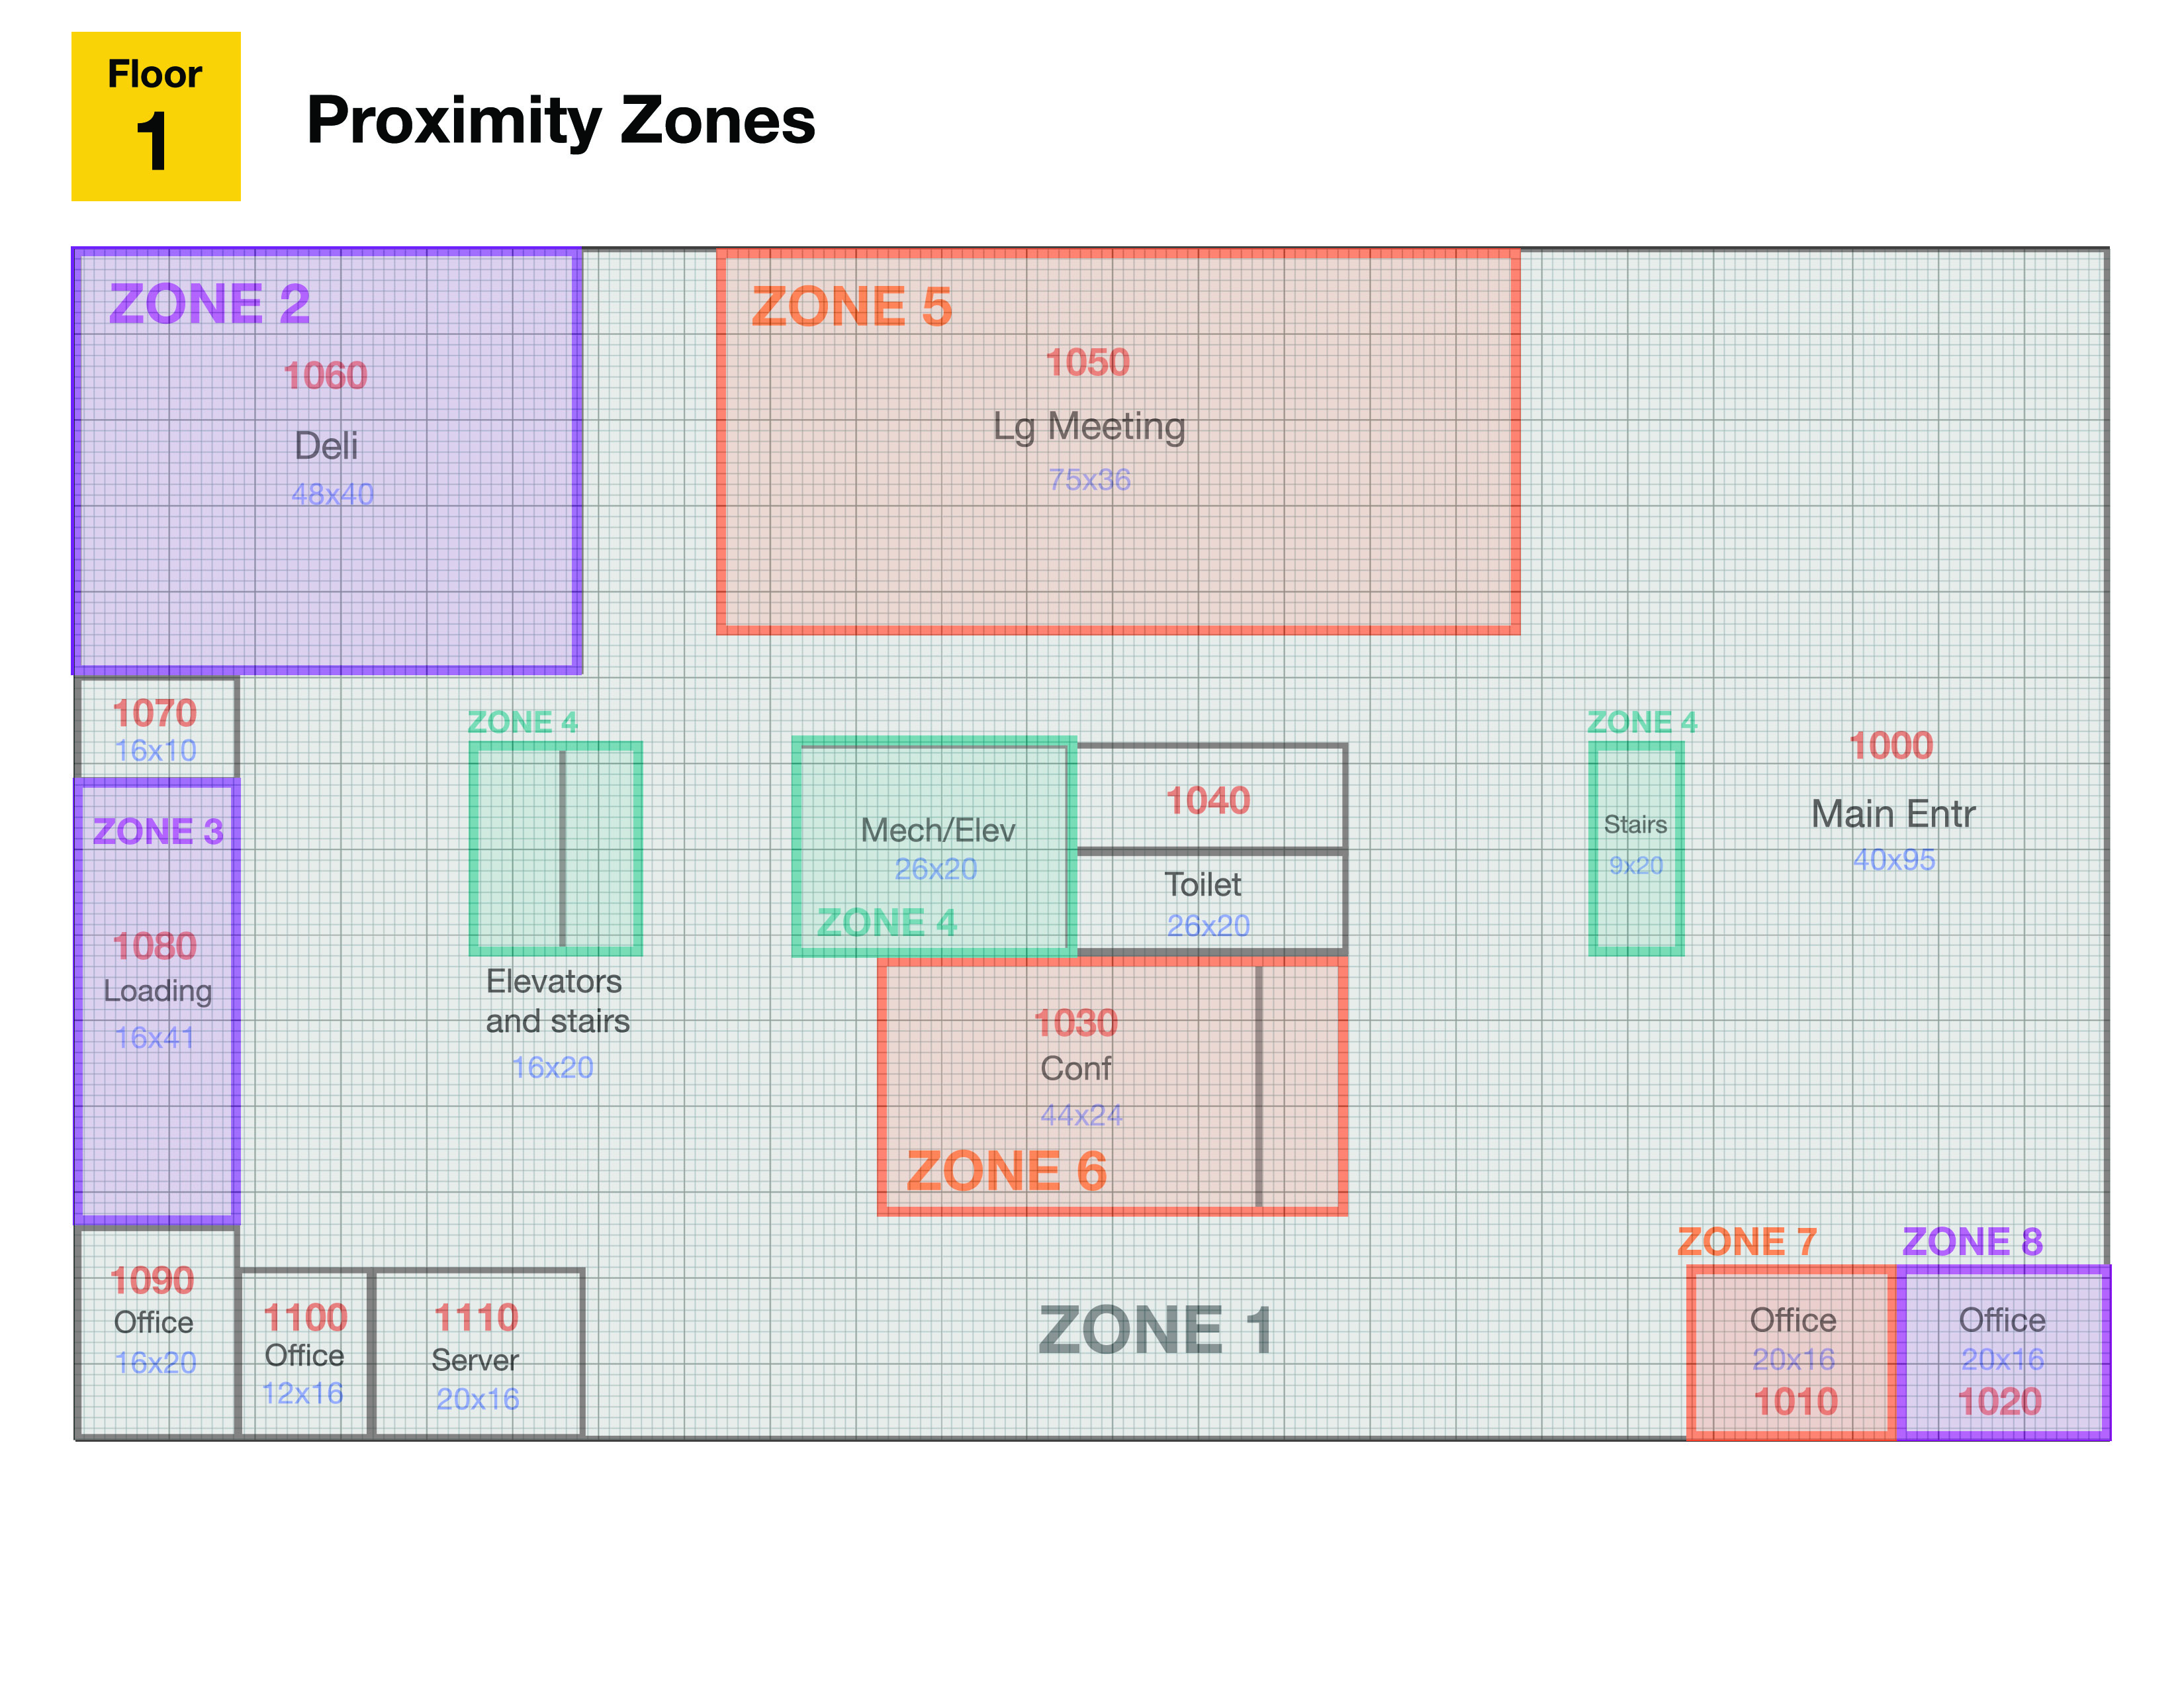
\includegraphics[width=0.3 \linewidth]{figures/prox1.jpg}
                        &
                        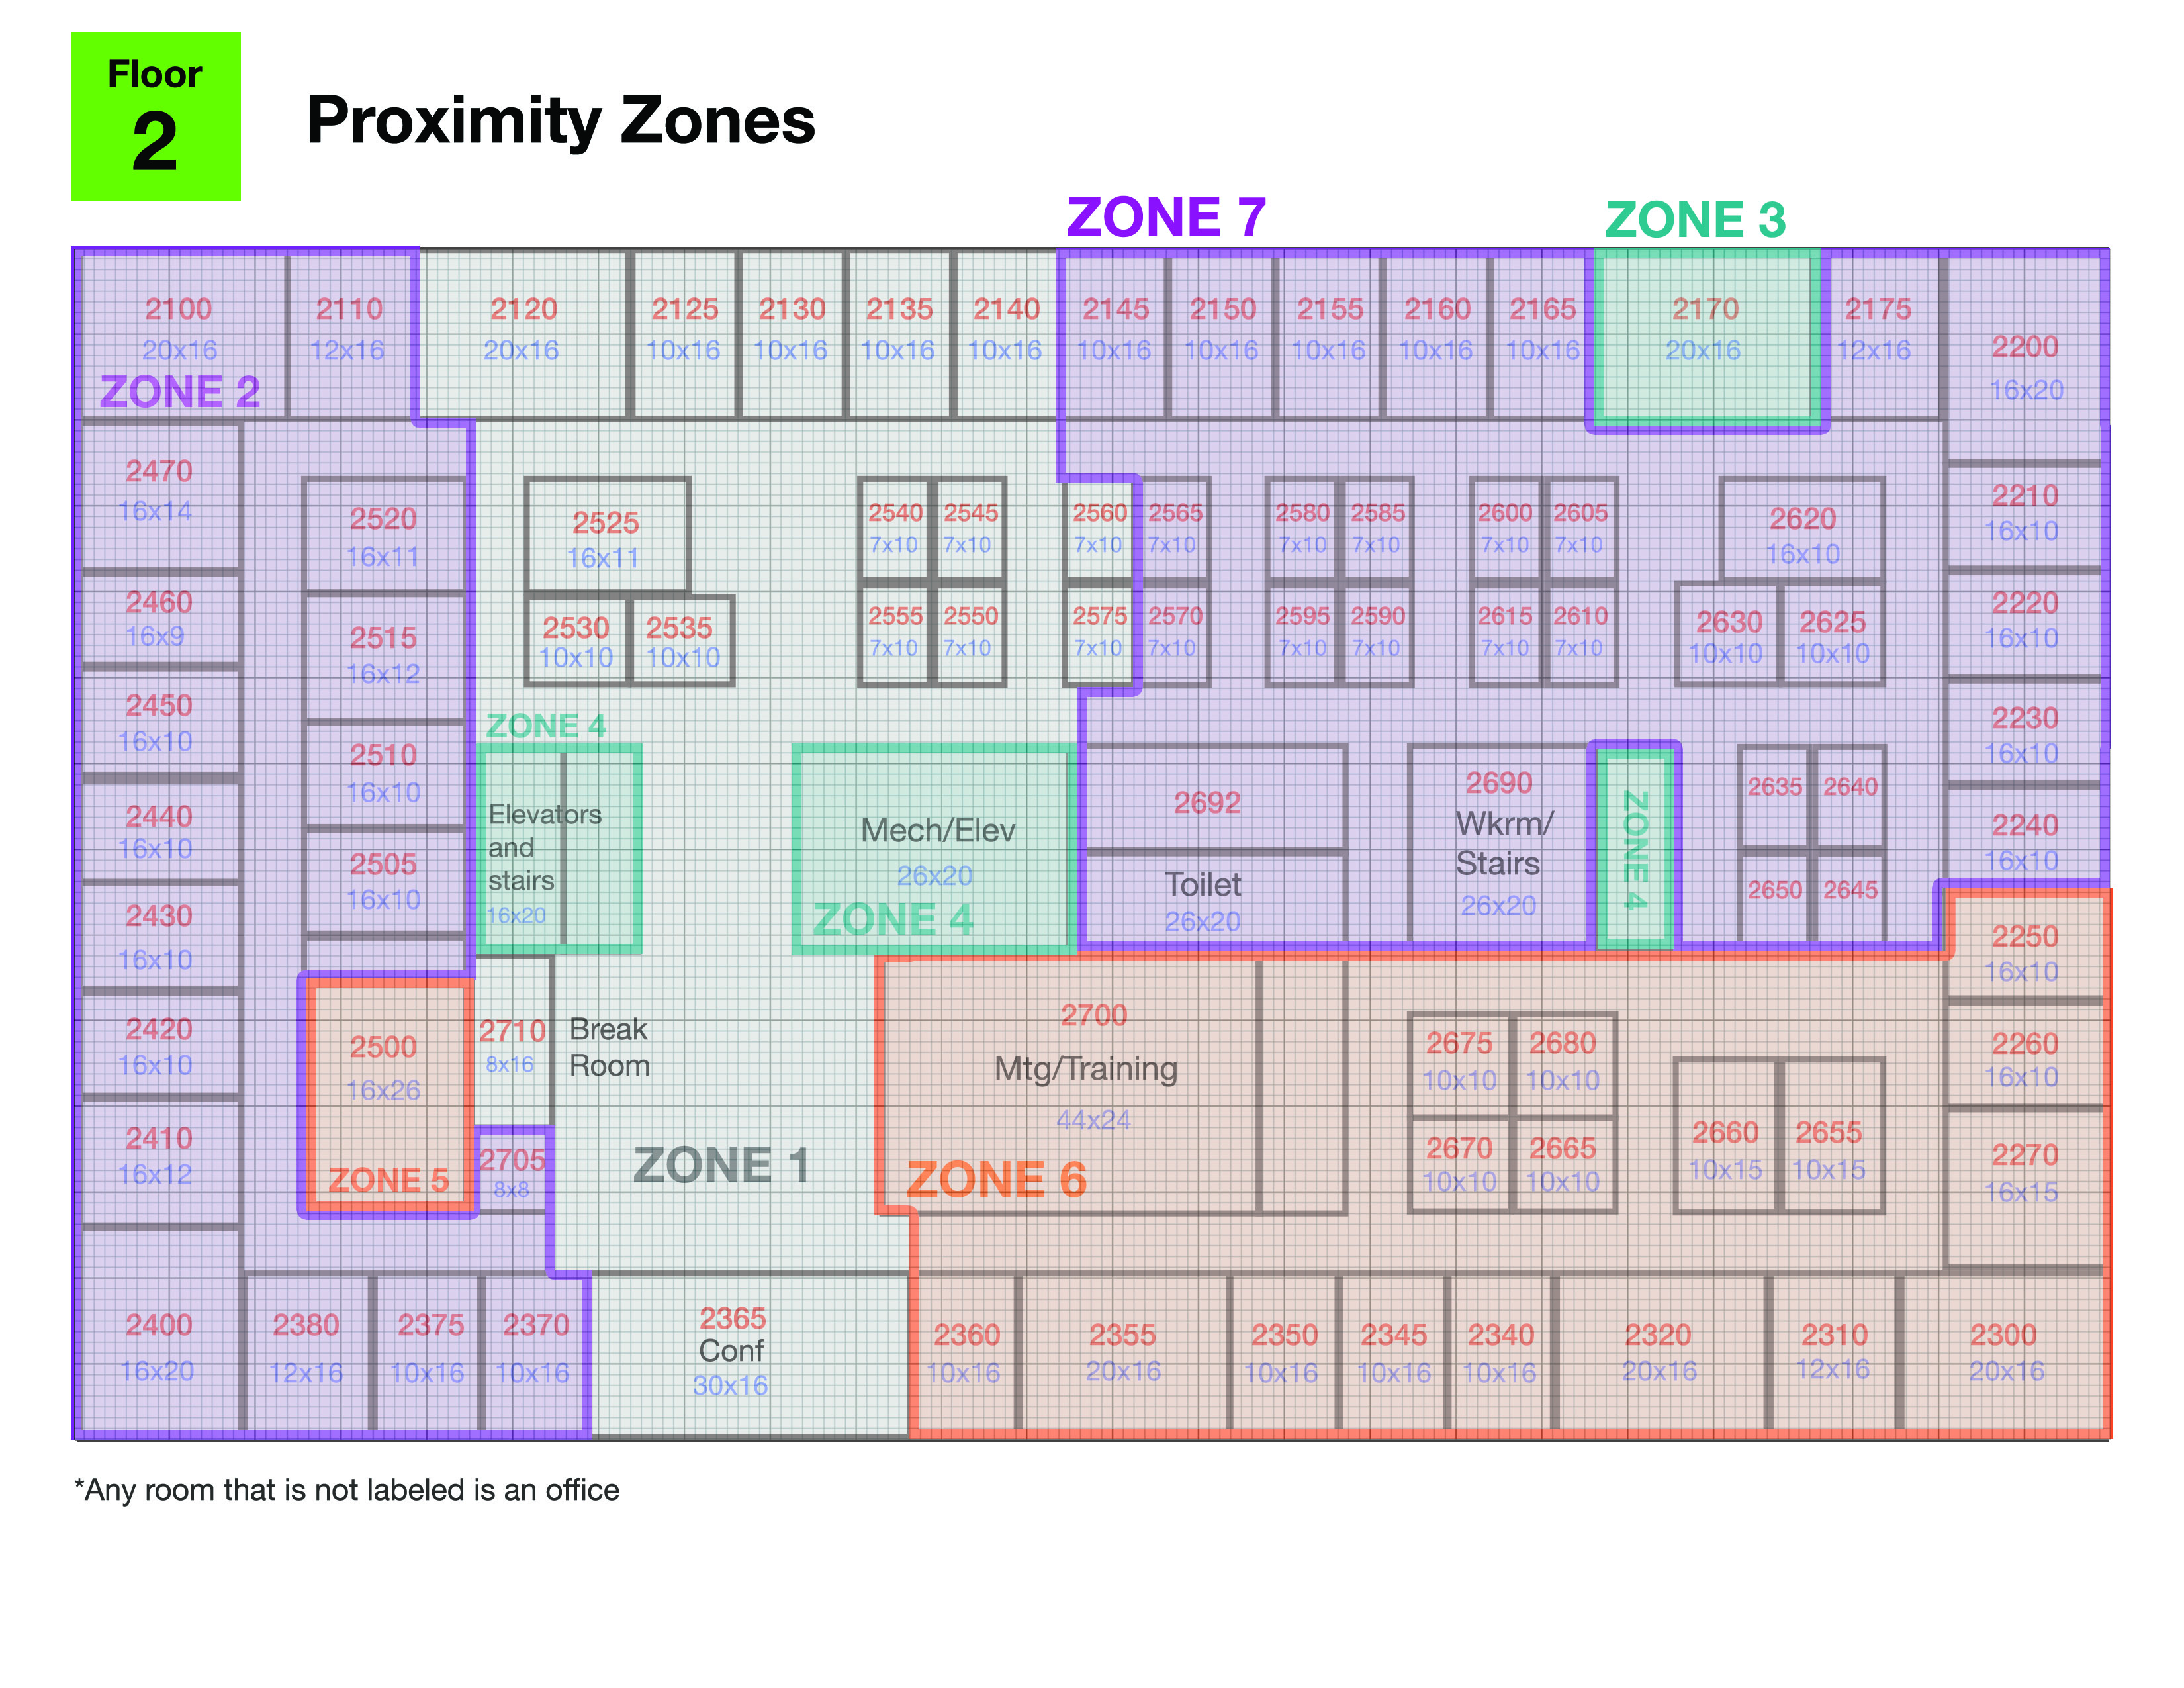
\includegraphics[width=0.3 \linewidth]{figures/prox2.jpg}
                        &
                        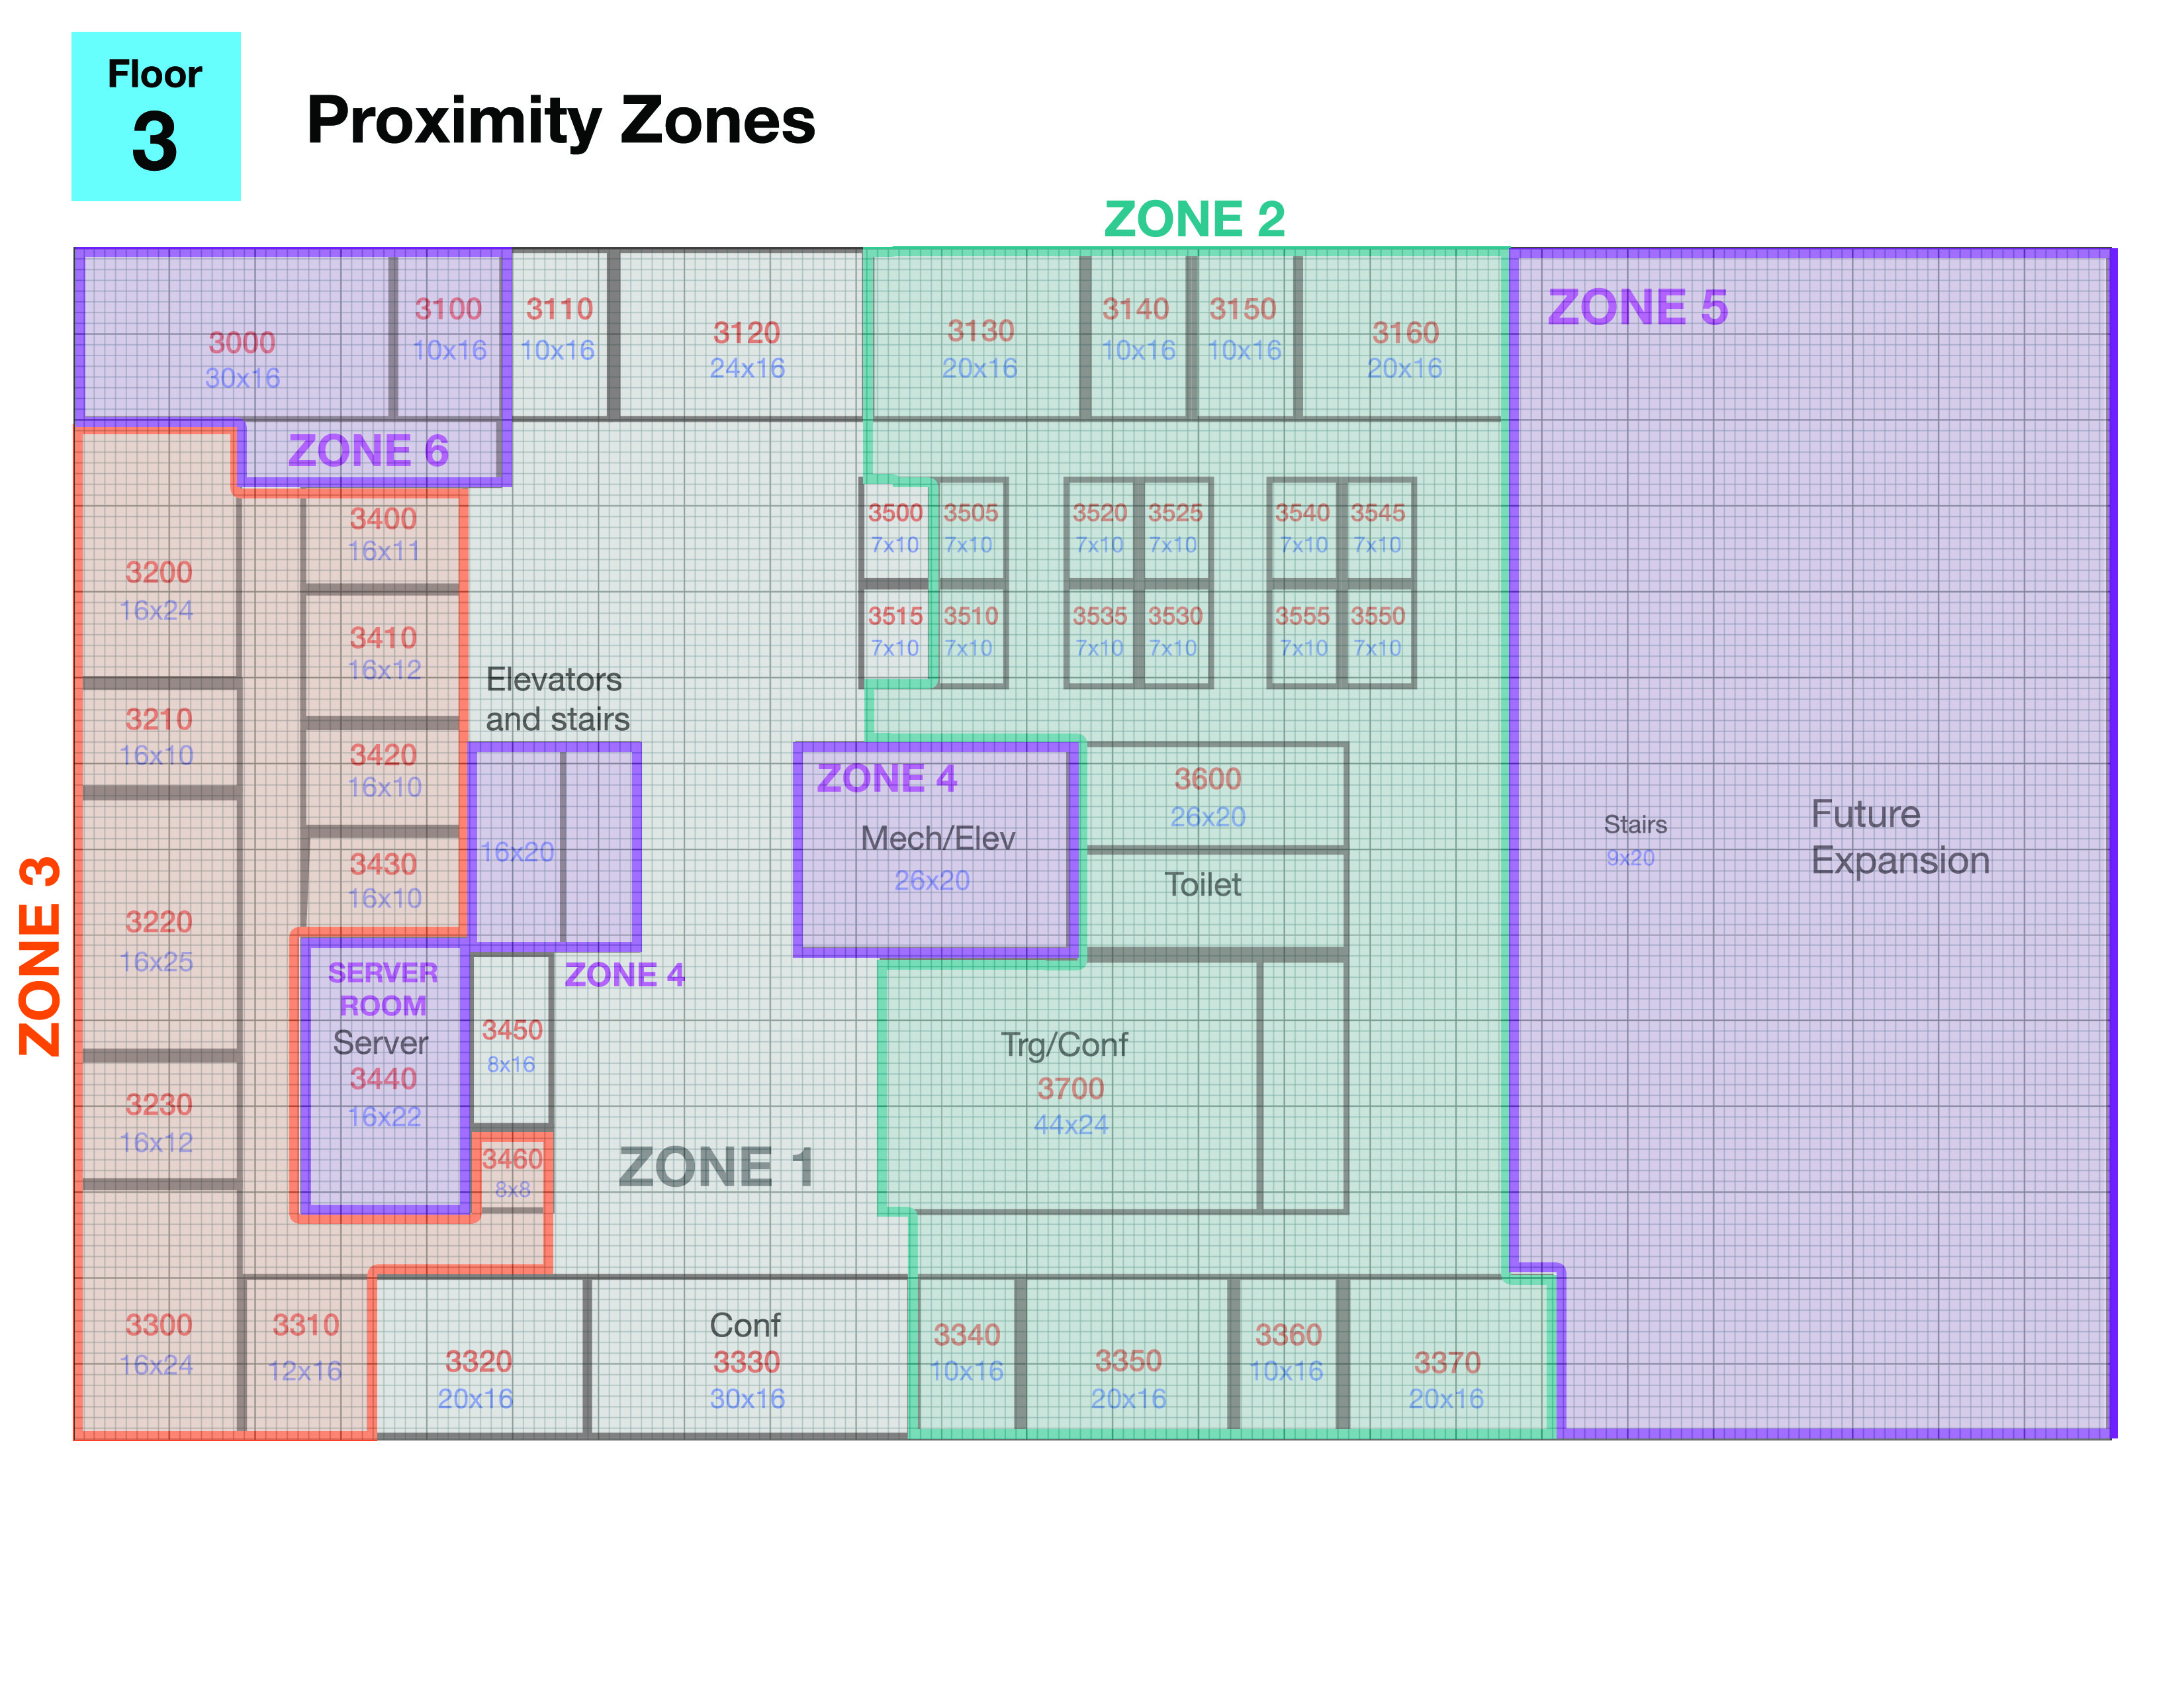
\includegraphics[width=0.3 \linewidth]{figures/prox3.jpg}
                        \\
                        
                        \mbox{(a) First Floor} & \mbox{(b) Second Floor} & \mbox{Third Floor} \\
                    \end{array}$
                    \caption{Prox zone of the Building}
                    \label{fig:prox}
                \end{figure}
            
                The prox zone of this building is as figure \ref{fig:prox}.
    
    \section{Methods}
    
    \section{Results}
        \subsection[Question 1]{What are the typical patterns in the prox card data? What does a typical day look like for GAStech employees? Describe up to five of the most interesting patterns that appear in the building data.}
            \subsubsection{Fixed prox data}
            
            \subsubsection{Mobile prox data}
        
        \subsection[Question 2]{Describe up to five of the most interesting patterns that appear in the building data. Describe what is notable about the pattern and explain its possible significance.}
        
        \subsection[Question 3]{Describe up to five notable anomalies or unusual events you see in the data. Prioritize those issue that are most likely to represent a danger or a serious issue for building operations.}
        
        \subsection[Question 4]{Describe up to three observed relationships between the proximity card data and building data elements. If you find a causal relationship, describe your discovered cause and effect, the evidence you found the support it, and your level of confidence in your assessment of the relationship.}
    
    \section{Discussion}
    
    \bibliographystyle{apacite}
    \bibliography{reference}
\end{document}